% !TeX encoding=utf8
% !TeX spellcheck = de_CH_frami

%
% add files for appendix chapter here


%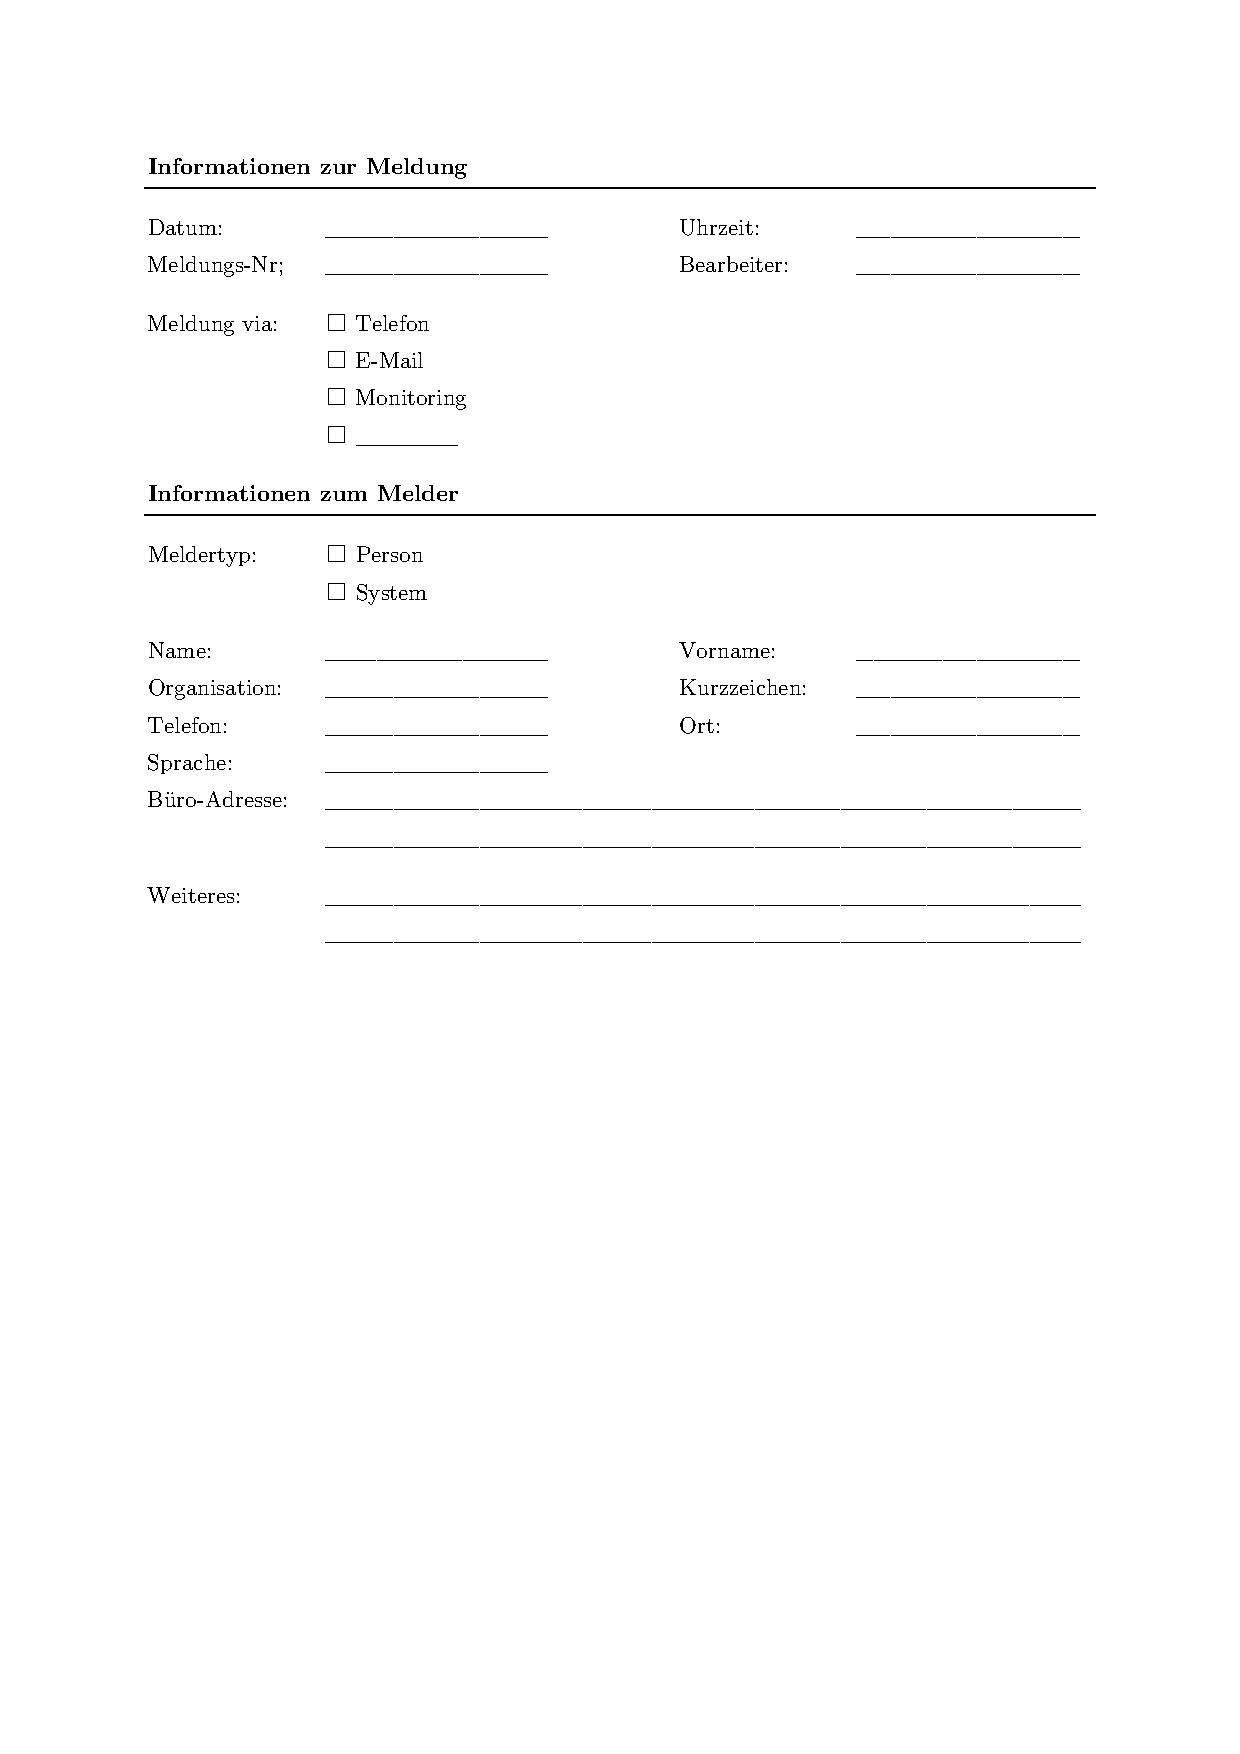
\includepdf[pages=-,picturecommand*={\put(133,660)\chapter{Vorlage: Formular Incident-Meldung} \label{appx:Template:IncidentMessage}}}]{content/appendix/Appendix_A_Formular_Incident_Meldung.pdf}
     
%\chapter{Vorlage: Formular Incident-Meldung}\label{appx:Template:IncidentMessage}

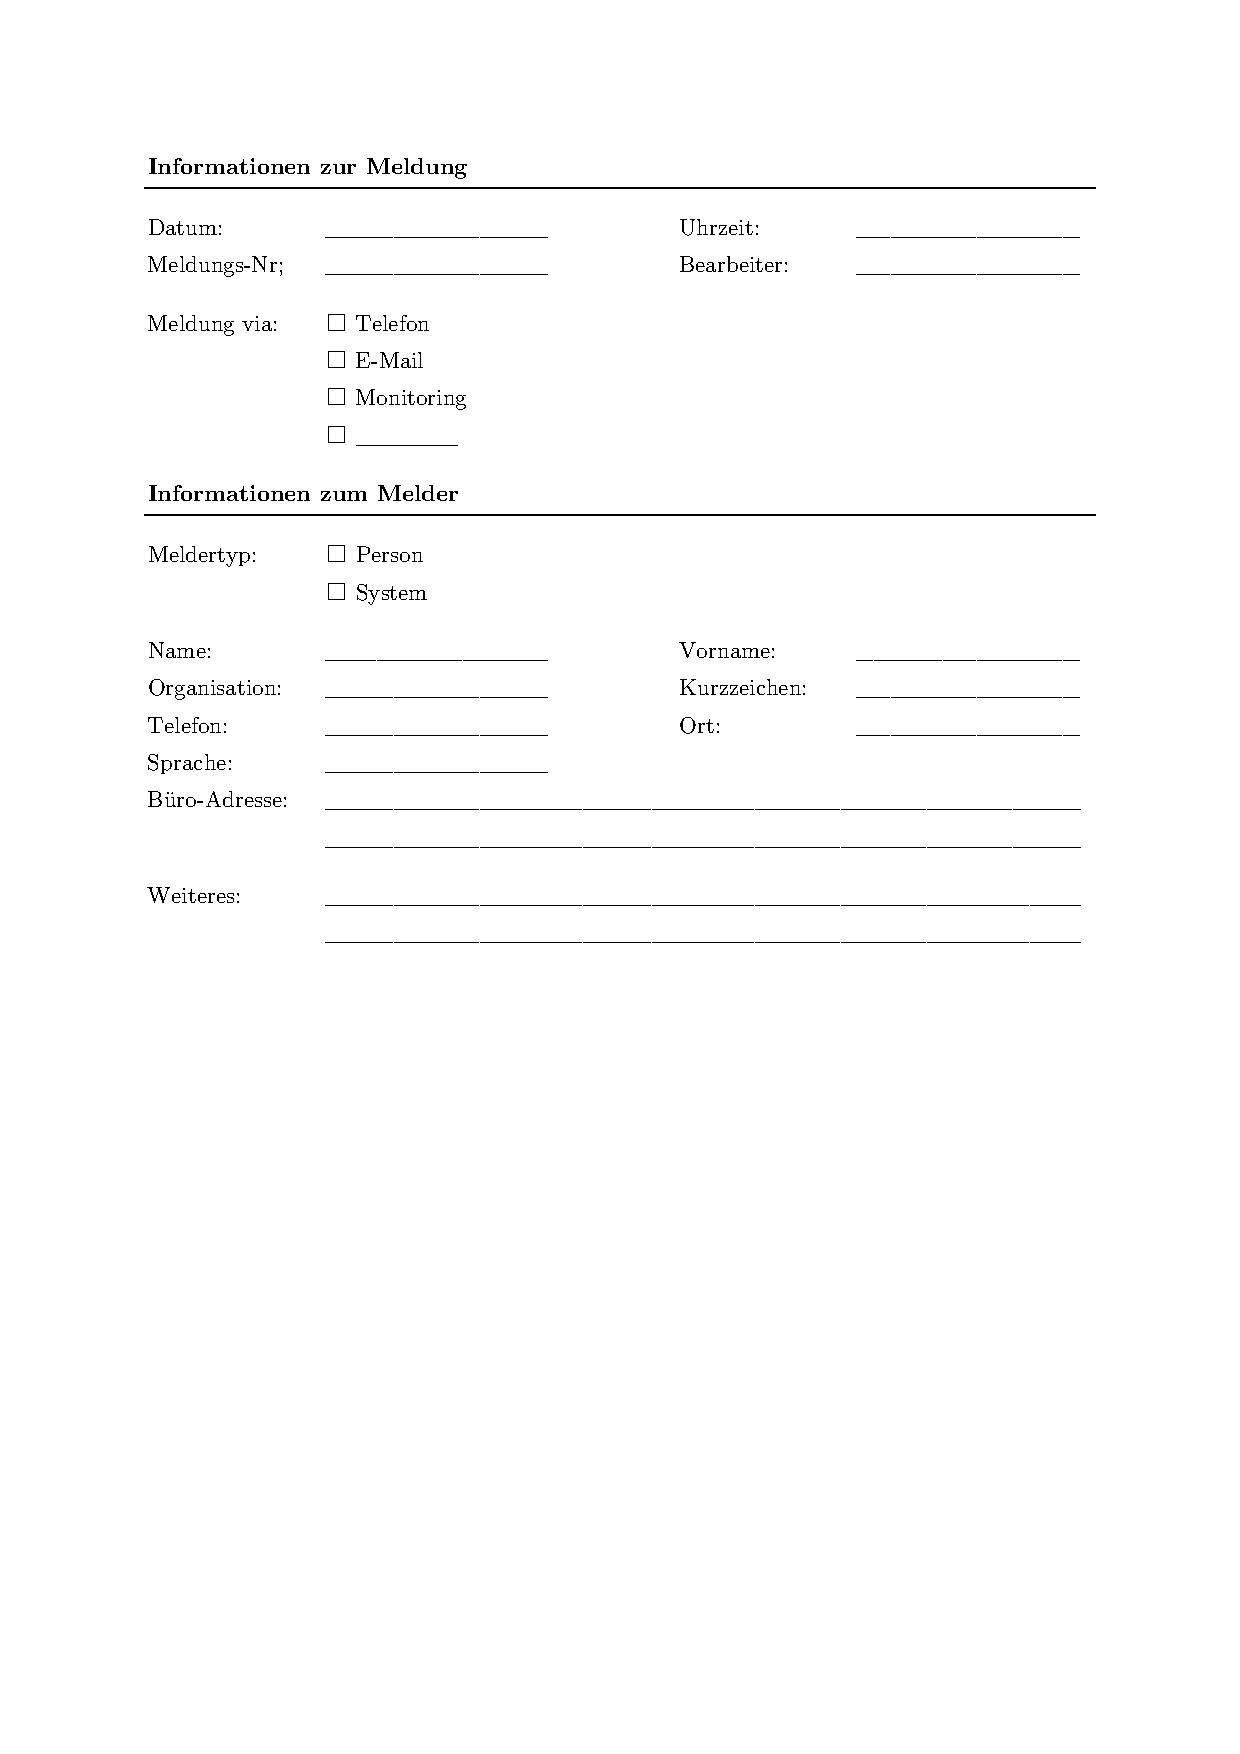
\includepdf[pages=1,noautoscale=true,scale=0.9,fitpaper=true, offset=-0.6cm -7cm,pagecommand={\chapter{Vorlage: Formular Incident-Meldung}\label{appx:Template:IncidentMessage}}]{content/appendix/Appendix_A_Formular_Incident_Meldung.pdf}

\includepdf[pages=2-last,noautoscale=true,scale=0.9,fitpaper=true,pagecommand={\thispagestyle{plain}}]{content/appendix/Appendix_A_Formular_Incident_Meldung.pdf}

\chapter{Vorlage Formular Ermittlung}
-Fallnummer
-Datum / Zeit
-Wieso forensische untersuchung (Verdacht?)
-Grund
-Ermittlungsleiter
-Ermittlungsteam
-Betroffene Systeme / Geräte / Anwendungen 8(Seriennummern und interne Bezeichnung)
-Verantwortliche Administratoren
-Protokolle, Incident Meldung, Beweiszettel

Täterprofil
-Was waren / sind mögliche Ziele
-Was ist der Grund für den Angriff / Einbruch?
-(Interne) komplizen?
-Tools / Techniken?
-Spuren?
....
\chapter{Vorlage: Protokoll}


Tabelle mit : Laufnummer, Zeit, Befehl / Aktion, Hash Ergebnisdatei, Kommentar
CF Seite 84

\chapter{Vorlage: Beweiszettel} \label{appx:Template:ProofPaper}
Buch CF: Seite 85

Beweiskette:

Laufwerke: Manufacturer, Model, Serial Number, Evidence Description (Name of suspect, Technologie: SATA, IDE, ...)





\chapter{Ablauf einer forensischen Analyse}
